\section{Performance Characterization and Known Issues}
\label{sec:performance}
%
In this section, we provide an assessment of the \gls{DP1} data quality and known issues.
% A summary of the Rubin \gls{DP1} key numbers and data quality metrics  is found in PERFSUMMARYTABLE
%%%%%% This table is auto generated from data, DO NOT EDIT
\startlongtable
\begin{deluxetable*}{llcccccccc}
\caption{Rubin Observatory Data Preview 1 Key Numbers \label{tab:dp1_key_numbers}}
% \tablecolumns{8}
% \tablenum{1}
% \tablewidth{0pt}
% %\tabletypesize{\scriptsize}
\tablehead{
    \colhead{head1} &
    \colhead{head2} &
    \colhead{fdsafdsa} &
    \colhead{fdsafdsa} &
    \colhead{fdsafdsa} &
    \colhead{fdsafds} &
    \colhead{fdsafds} &
    \colhead{}
}
\startdata
    432432 & 32432432 & 43243243 & 432  & 432432  & 543232  & 54332  & 5432543 \\
\enddata
\end{deluxetable*}


\subsection{Sensor Anomalies and ISR}
\label{ssec:sensor_anomalies}
In addition to the known detector features identified before LSSTComCam commissioning, most of which are handled by the ISR processing (see \secref{ssec:isr}), we discovered a number of new types of anomalies in the DP1 data. 
Since no corrections are currently available for these anomalies, they are masked and excluded from downstream data products.

\subsubsection{Vampire Pixels}
Vampire pixels are visible on the images as a bright defect surrounded by a region of depressed flux, as though the defect is stealing charge from its neighboring pixels; they have been termed ``vampire'' defects.
 \figref{fig:anomalies_vampire_pixels}  shows an example of a vampire pixel near the center of R22\_S11 on an r-band flat.

From studies on evenly illuminated images, vampires appear to conserve charge.
Unfortunately, there's no clean way to redistribute this stolen flux, and so we have identified as many of them as possible and created manual defect masks to exclude them from processing.
We have found some similar features on the ITL detectors on LSSTCam, and will use the same approach to exclude them.
\begin{figure}[htb!]
  \centering
  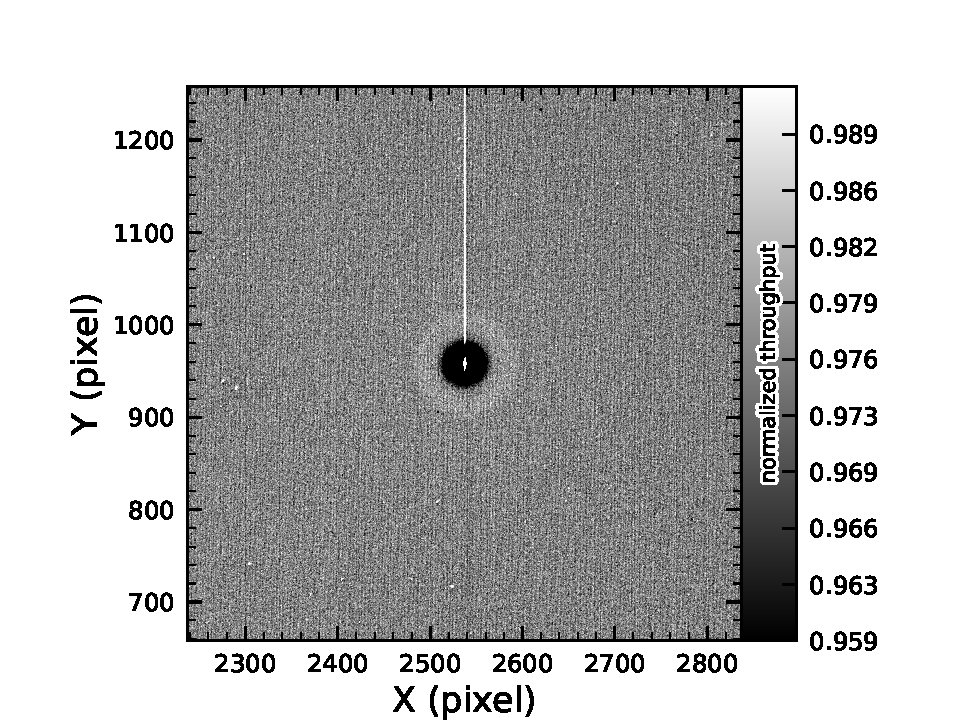
\includegraphics[width=0.98\linewidth]{figures/dp1_isr_anomalies-vampire_pixel.pdf}
  \caption{A large \textit{vampire pixel} near the center of R22\_S11, as seen on the r-band flat.}
   \label{fig:anomalies_vampire_pixels}
\end{figure}

\subsubsection{Phosphorescence}
Some regions were seen to contain large numbers of bright defects.
An example is shown in   \figref{fig:anomalies_phosphorescence}  in a g-band flat. 
On closer study, it appears that on some detectors a layer of photoresist wax was incompletely removed from the detector surface during production.
As this wax is now trapped below the surface coatings, there is no way to physically clean these surfaces.
If this wax responded to all wavelengths equally, then it would likely result in quantum efficiency dips, which might be removable during flat correction.
However, it appears that this wax is slightly phosphorescent, with a decay time on the order of minutes, resulting in the brightness of these sources being dependent on the illumination of prior exposures.
The worst of these regions were excluded with manual masks, but we do not expect to need to do this for LSSTCam.
\begin{figure}[htb!]
  \centering
  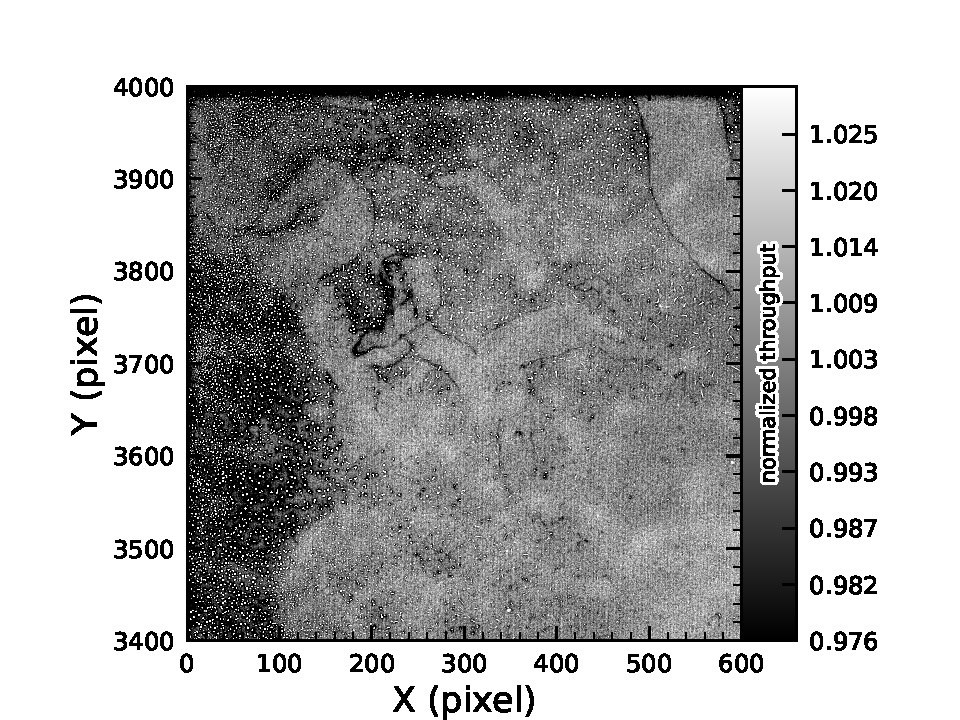
\includegraphics[width=0.98\linewidth]{figures/dp1_isr_anomalies-phosphorescence.pdf}
  \caption{The top left corner of R22\_S01 in the g-band flat, showing the many small defect features that are caused by the remnant photoresist wax.
  A single large defect box masks this region from further analysis to prevent these features from contaminating measurements.}
  \label{fig:anomalies_phosphorescence}
\end{figure}

\subsubsection{Crosstalk}
We use an average crosstalk correction based on laboratory measurements with LSSTCam.
These average corrections performed better than expected, and so have been used as-is for DP1 processing.
There are, however, some residual crosstalk features present post-correction, with a tendency towards over-subtraction.
\figref{fig:crosstalk_residual} shows an example  of a bright star with over-subtracted crosstalk residuals visible on neighboring amplifiers to both sides on exposure 2024120600239, detector R22\_S02.
\begin{figure}[htb!]
  \centering
  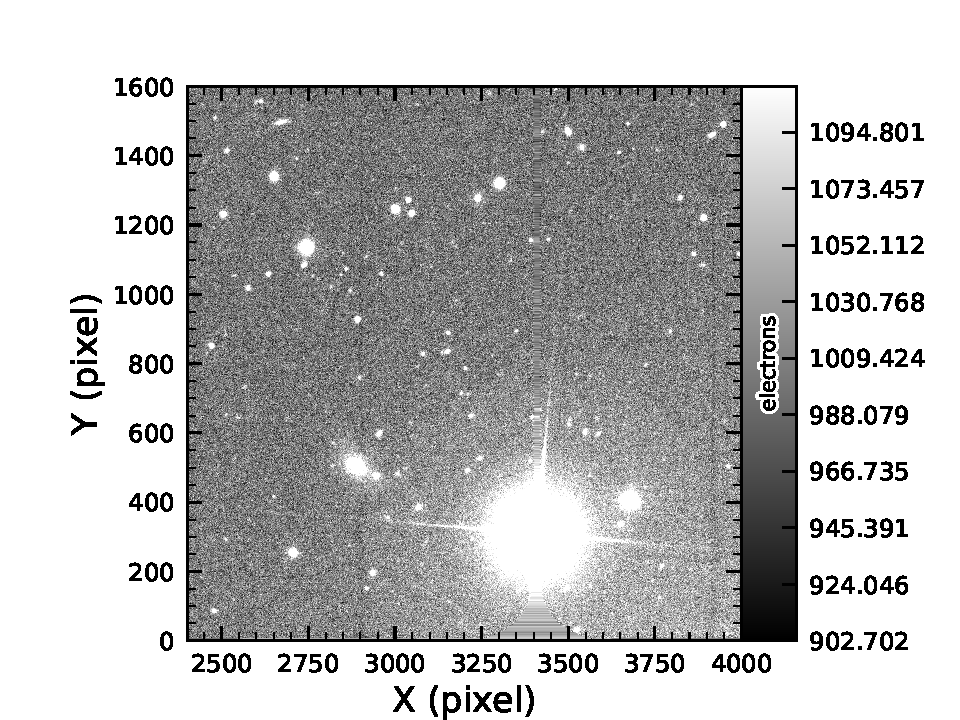
\includegraphics[width=0.98\linewidth]{figures/dp1_isr_anomalies-crosstalk_residual.pdf}
  \caption{An example of a bright star with over-subtracted crosstalk residuals visible on neighboring amplifiers to both sides (exposure 2024120600239, detector R22\_S02).
  The horizontal banding stretching from the center of the star shows the interpolation pattern covering the saturated core and the ITL edge bleed near the serial register.}
  \label{fig:crosstalk_residual}
\end{figure}

\subsubsection{Bleed Trails}
Bleed trails from saturated sources were expected on LSSTComCam, but they appear in more dramatic forms than was expected.
As a bleed trail nears the serial register, it fans out into a ``trumpet'' shaped feature.
Although bright, these features do not have consistently saturated pixels.
In DP1 these ``edge bleeds'' were programmatically identified and masked.

Saturated sources can create a second type of bleed, where the central bleed drops below the background level.
The depressed columns along these trails extend across the entire height of the detector, crossing the detector mid-line.
We developed a model for these to identify which sources are sufficiently saturated to result in such a trail, which is then masked.  As these kind of trails appear only on the ITL detectors, we've named these features ``ITL dips.''
\figref{fig:anomalies_itl_dip} shows an example of a   bright star exhibiting the ``ITL dip'' phenomenon on exposure: 2024121000503, detector: R22\_S21.
\begin{figure}[htb!]
  \centering
  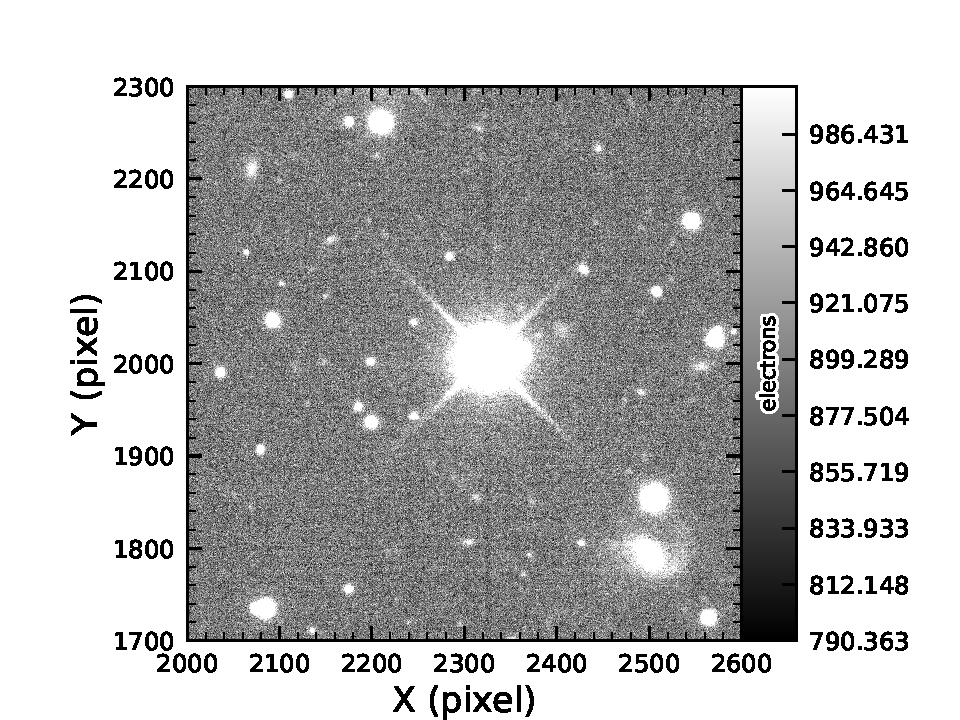
\includegraphics[width=0.98\linewidth]{figures/dp1_isr_anomalies-itl_dip.pdf}
  \caption{A bright star showing the ``ITL dip'' phenomenon, in which a dark trail extends out from the star to the top and bottom edges of the detector (exposure: 2024121000503, detector: R22\_S21).}
\label{fig:anomalies_itl_dip}
\end{figure}



\subsection{PSF Models}
\label{ssec:psf_models}
To characterize \gls{PSF}  performance, we use adaptive second moments \citep{2002AJ....123..583B} measured on \gls{PSF} stars and on the PSF model using the \gls{HSM} implementation \citep{2003MNRAS.343..459H, 2005MNRAS.361.1287M}.
All measurements are expressed in the pixel coordinate frame of each detector.
We characterize the performance of the PSF using the classical trace of the  second moment matrix $T$, along with the ellipticity parameters $e^1$ and $e^2$.
Measurements on the observed PSF stars are are denoted as  $T_{\text{PSF}}$, $e^1_{\text{PSF}}$,  $e^2_{\text{PSF}}$, while those from PSF models are denoted as  $T_{\text{model}}$, $e^1_{\text{model}}$, $e^2_{\text{model}}$.
We compare two PSF modeling approaches:
\begin{itemize}
\item Piff with second-order polynomial interpolation (Piff O2), the pipeline's default, and
\item Piff with fourth-order polynomial interpolation (Piff O4), which serves as the final DP1 PSF model.	
\end{itemize}
\tabref{tab:psf-1d_stats} summarizes each model’s ability to reconstruct the mean $T$, $e^1$, and $e^2$ on  \gls{LSSTComCam}. 
Both models exhibit a negative residual bias in the reconstructed PSF size, with Piff O4 providing improved performance over Piff O2.
\begin{deluxetable*}{lccc}
\caption{Comparison of observed and model residuals, across all visits and filters.}
\label{tab:psf-1d_stats}
\tablehead{
  \colhead{\textbf{Quantity}} & 
  \colhead{\textbf{Observed}} & 
  \colhead{\textbf{Piff O2}} & 
  \colhead{\textbf{Piff O4}} \\
  \colhead{} & 
  \colhead{} & 
  \colhead{$\times10^{-4}$} & 
  \colhead{$\times10^{-4}$} 
}
\startdata
$\langle T\rangle\ (\mathrm{pixel}^2)$ & $11.366 \pm 0.003$ & & \\
$\langle e^1\rangle$ & $(-6.07\pm0.05)\times10^{-3}$ & & \\
$\langle e^2\rangle$ & $(-4.57\pm0.05)\times10^{-3}$ & & \\
$\langle e\rangle$ & $(8.794\pm0.004)\times10^{-2}$ & & \\
$\langle \delta T / T\rangle$  & & $-4.0\pm0.2$ & $-5.0\pm0.2$ \\
$\langle \delta e^1\rangle$ & & $0.6\pm0.1$ & $0.5\pm0.1$ \\
$\langle \delta e^2\rangle$ & & $0.0\pm0.1$ & $0.0\pm0.1$ \\
\enddata
\end{deluxetable*}

% \begin{table}[ht]
%   \centering
%   \caption{Comparison of observed and model residuals, across all visits and filters.}
%   \label{tab:psf-1d_stats}
%   \begin{tabular}{l c c c}
%     \toprule
%     & Observed 
%     & Piff (order 2) 
%     & Piff (order 4) \\
%     \midrule
%     $\langle T\rangle\ (\mathrm{pixel}^2)$ 
%       & $11.366 \pm 0.003$ 
%       & 
%       & 
%     \\[4pt]
%     $\langle e^1\rangle$ 
%       & $(-6.07\pm0.05)\times10^{-3}$ 
%       & 
%       & 
%     \\[4pt]
%     $\langle e^2\rangle$ 
%       & $(-4.57\pm0.05)\times10^{-3}$ 
%       & 
%       & 
%     \\[4pt]
%     $\langle e\rangle$ 
%       & $(8.794\pm0.004)\times10^{-2}$
%       & 
%       & 
%     \\[8pt]
%     $\langle \delta T / T\rangle$ 
%       & 
%       & $(-4.0\pm0.2)\times10^{-4}$ 
%       & $(-5.0\pm0.2)\times10^{-4}$
%     \\[4pt]
%     $\langle \delta e^1\rangle$ 
%       & 
%       & $(0.6\pm0.1)\times10^{-4}$ 
%       & $(0.5\pm0.1)\times10^{-4}$
%     \\[4pt]
%     $\langle \delta e^2\rangle$ 
%       & 
%       & $(0.0\pm0.1)\times10^{-4}$ 
%       & $(0.0\pm0.1)\times10^{-4}$
%     \\
%     \bottomrule
%   \end{tabular}
% \end{table}

An alternative approach to evaluating the performance of the \gls{PSF} model is to examine the average $\delta T/T$, where $\delta T$ is $T_{\text{PSF}}$ - $T_{\text{model}}$, across visits, projected onto focal-plane coordinates, as shown in \figref{fig:psf_residuals_fov}. 
Piff reveals strong spatial correlations in the residuals, including a systematic offset consistent with the results presented in \tabref{tab:psf-1d_stats}. 
The presence of these spatial structures motivated the adoption of fourth-order polynomial interpolation in all bands except $u$-band. 
Although not shown in \figref{fig:psf_residuals_fov}, residual patterns persist even with third-order interpolation, indicating that it is insufficient to capture the complexity of the PSF variation. 
Increasing the interpolation order to five would nominally reduce the residuals further, but the limited number of stars available on some CCDs would not provide adequate constraints for such a model, while the resulting improvement would likely be minimal.
Preliminary analysis of LSSTCam data in the laboratory at \gls{SLAC} shows that the \gls{ITL} sensors exhibit the same pattern as \gls{ITL} sensors on \gls{LSSTComCam}.
%The sensors' $\delta T/T$ is fully correlated with the height variation across the LSSTCam \gls{ITL} sensors, which explains this behavior.
%Future data processing will account for this height variation directly in the \gls{PSF} model.
\begin{figure*}[htb!]
\centering
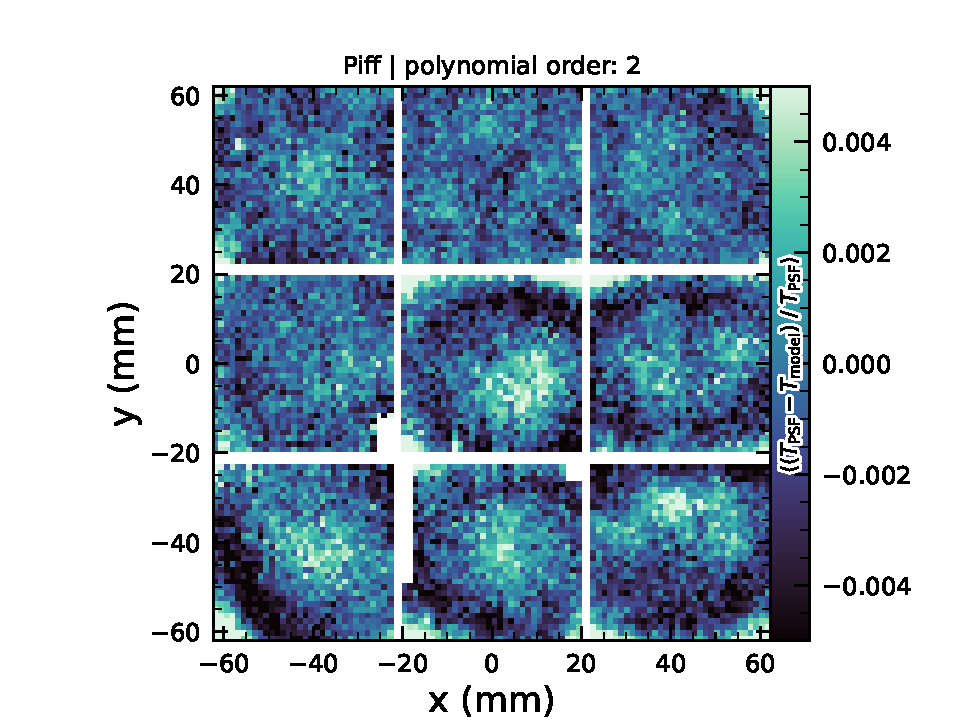
\includegraphics[scale=0.45]{dT_T_Piff_poly_order_2}
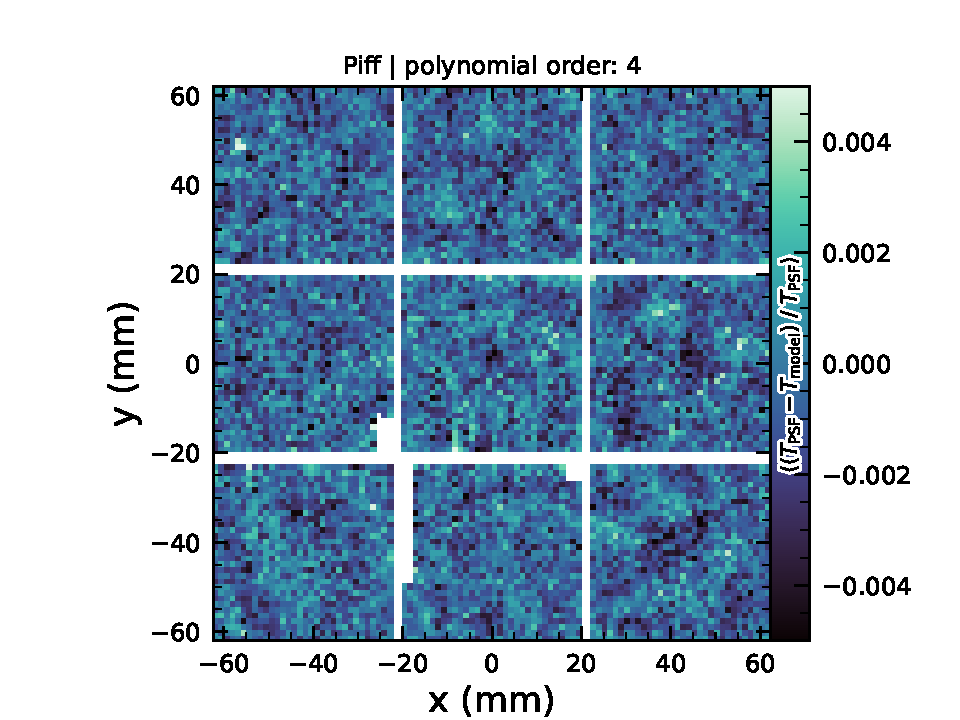
\includegraphics[scale=0.45]{dT_T_Piff_poly_order_4}
\caption{\small Average across all visits of $\delta T/T$  for Piff O2 and Piff O4 modeling on \gls{LSSTComCam}. Averages are computed using a 120x120 binning.}
\label{fig:psf_residuals_fov}
\end{figure*}

Another way to look at the \gls{PSF} modeling quality is via whisker plots of the \gls{PSF} second and fourth moments and their modeling residuals projected on a part of the sky.
In addition to the second moment, the spin-2 fourth moments, $e^{(4)}$, are defined as:
\begin{align*}
e^{(4)}_1 &= M_{\text{40}} - M_{\text{04}} \\
e^{(4)}_2 &= 2\left(M_{\text{31}} - M_{\text{13}}\right),
\end{align*}
where $M_{\text{pq}}$ are the standardized higher moments as defined in \cite{2023MNRAS.520.2328Z} measured on stars and PSF models.
\figref{fig:psf_residuals_whisker_ECDFS} shows
the whisker plots of $e$, $e^{(4)}$ (top rows), and $\delta e$, $\delta e^{(4)}$
in the \gls{ECDFS} field. 
The direction of a whisker represents the orientation of the \gls{shape}, while the length represents the amplitude $|e|$ or $|e^{(4)}|$.
We observe coherent patterns in both the \gls{PSF} moments and the residuals, the latter of which warrants further investigation if it persists in future data releases.
\begin{figure}[htb!]
    \centering
    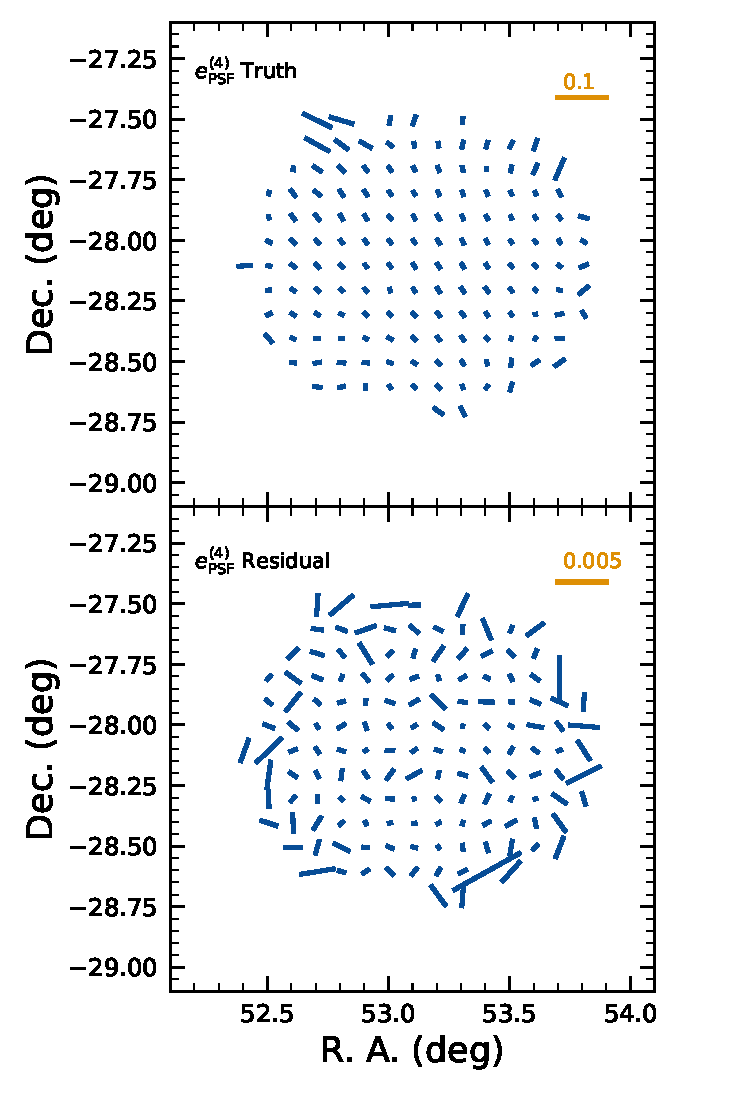
\includegraphics[scale=0.33]{psf_fourth_whisker}
    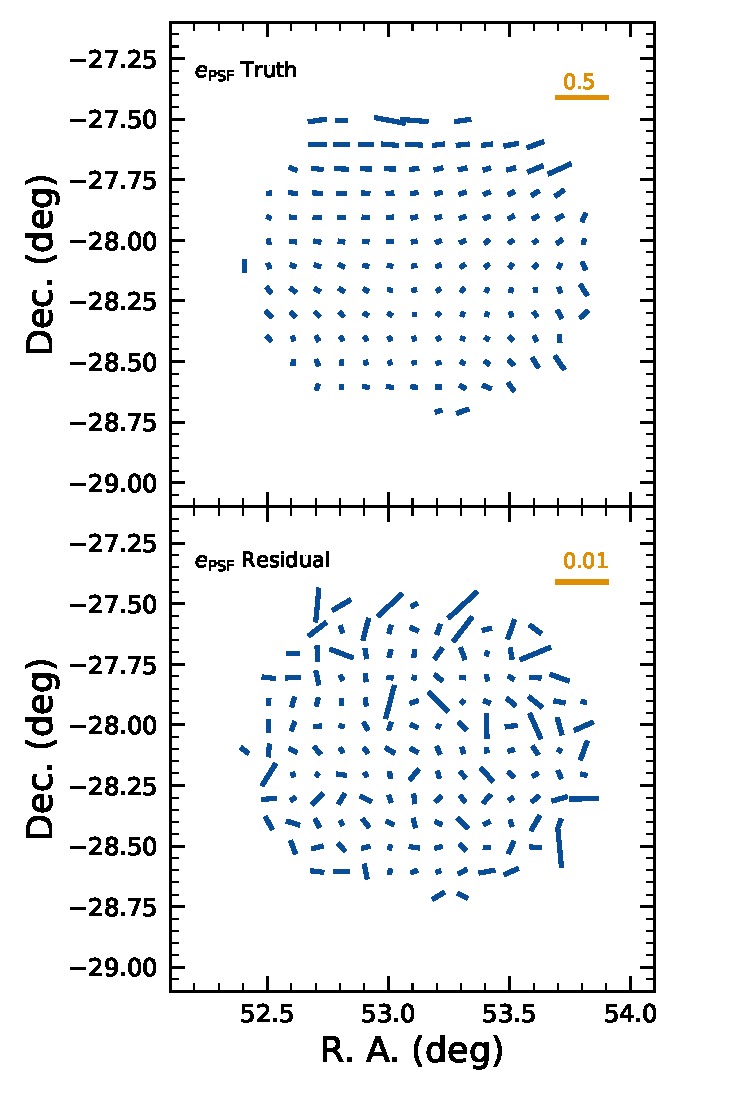
\includegraphics[scale=0.33]{psf_second_whisker}
    \caption{\small Whisker plots for the  \gls{ECDFS} field for $e$, $e^{(4)}$ and $\delta e$, $\delta e^{(4)}$.}
    \label{fig:psf_residuals_whisker_ECDFS}
\end{figure}›

\figref{fig:psf_residuals_mag_color} shows a plot of  $\delta T/T$ versus stellar magnitude, which can reveal any dependencies between \gls{PSF} size and flux.
We also repeat this analysis in color bins to probe chromatic effects.
Binning by color uncovers a clear color dependence, as was also seen in \gls{DES} \citep{DES:2020vau}.
The residual is consistent with \tabref{tab:psf-1d_stats} and its cause is unknown.
DP1 does not include the color correction implemented in the DES Year 6 analysis, \citet{2025OJAp....8E..26S}. 
This will be included in processing of future data releases.
\begin{figure}[htb!]
\plotone{dT_T_Piff_poly_4_vs_mag}
\caption{Binned $\delta T/T$ as a function of magnitude across all visits and filters and in bins of stellar colors.}
\label{fig:psf_residuals_mag_color}
\end{figure}

As noted in  \cite{PSTN-019}, two key Piff features were not used in the DP1 processing.
PSF color dependence was not implemented, and, while Rubin software allows Piff to work with sky coordinates (including WCS transformations), 
it does not yet correct for sensor-induced astrometric distortions such as tree rings \citep{2017JInst..12C5015P}.
Both features are planned for upcoming releases.

\subsection{Astrometry}
To characterize astrometric performance, we evaluate both internal consistency and agreement with an external reference.
The primary measure of internal consistency is the repeatability of position measurements for the same object, defined as the RMS of the astrometric distance distribution for 
stellar pairs having a specified separation in arcminutes. 
We associate isolated point sources across visits and compute the rms of their fitted positions, rejecting any stars with another star within  2\arcsec.
\figref{fig:dmAstroErr} shows the median per-\gls{tract} rms astrometric error in RA  for all isolated point sources, both after the initial calibration and after the final calibration, which includes proper motion corrections.
The results indicate that the astrometric solution is already very good after the initial \gls{calibration}.
Global calibration yields only modest improvement, likely due to the short time span of \gls{DP1} and the minimal distortions in the LSSTComCam.
In the main survey, the longer time baseline and greater distortions near the \gls{LSSTCam} field edges will make global calibration more impactful.
\begin{figure}[htb!]
\plotone{Astrometry_dmAstroErr}
\caption{Mean per-tract astrometric repeatability of measurements of isolated point sources in RA in visits across all bands.}
\label{fig:dmAstroErr}
\end{figure}
An additional measure of internal consistency is the repeatability of separations between objects at a given distance.
To compute this, we identify pairs of objects that are separated by a specified distance and measure their precise separation during each visit in which both objects are observed.
The scatter in these separation measurements provides an indication of the internal consistency of the astrometric model.
\figref{fig:AM1} shows the median separation for pairs of objects separated by approximately 5 arcminutes, computed per tract after the final calibration.
\begin{figure}[htb!]
\plotone{Astrometry_AM1}
 \caption{Median per-tract repeatability in separations between isolated point sources 5~arcmin apart in visits across all bands.}
 \label{fig:AM1}
 \end{figure}
These values are already approaching the design requirement of $10$ mas.

To assess external consistency, we consider the median separation between sources not included in the astrometric fit and associated objects from a reference catalog.
For this, we use the Gaia \gls{DR3} catalog, with the object positions shifted to the observation epoch using the Gaia proper motion parameters.
\figref{fig:AA1} shows the median separation for each visit in the $r$-band in \gls{tract} 4849 in the ECDFS fields (\tabref{tab:dp1_tracts}).
\begin{figure*}[htb!]
\plotone{Astrometry_AA1}
\caption{Median absolute offset for all visits in $r$-band in \gls{tract} 4849 in the ECDFS field. 
The offset is the difference between the positions of isolated point sources that were reserved from the astrometric fit and matched objects from the Gaia DR3 catalog.}
\label{fig:AA1}
\end{figure*}
The calculated values are almost all within $5$\xspace mas, well below the design requirement of $50$\xspace mas for the main survey.
By examining the astrometric residuals, we can assess whether there are distortions not accounted for by the astrometric model. 
In some cases, residuals from a single visit exhibit behavior consistent with atmospheric turbulence, as shown in \figref{fig:Astrometry_Emode}, which is characterized by a curl-free gradient field in the two-point correlation function of the residuals (E-mode),  \citet{Leget2021} and \citet{Fortino2021}. 
\begin{figure*}[htb!]
\plotone{Astrometry_2024120200359}
\caption{Astrometric residuals in $u$ (left panel) and $v$ (center panel) directions with the E (blue) and B (orange) modes of the two-point correlation function (right panel) 
seen in visit 2024120200359 in tract 2393 in $u$ band.
The residuals show a wave-like pattern characteristic of atmospheric turbulence, and there is significant E-mode and negligible B-mode in the correlation function.}
\label{fig:Astrometry_Emode}
\end{figure*}
However, as seen in \figref{fig:Astrometry_EBmode}, the residuals in many visits also have correlation functions with a non-negligible divergence-free B-mode,
indicating that some of the remaining residuals are due to unmodeled instrumental effects, such as rotations between visits.
\begin{figure*}[htb!]
\plotone{Astrometry_2024120700527}
\caption{Astrometric residuals in $u$ (left panel) and $v$ (center panel) directions, with the E (blue)  and B (orange) 
modes of the two-point correlation function (right panel) seen in visit 2024120700527 in tract 2393 in $u$ band.
There are coherent residuals, but without the wave-like pattern seen in \figref{fig:Astrometry_Emode}, and the correlation function has significant values for both E and B-modes.}
\label{fig:Astrometry_EBmode}
\end{figure*}

We can see unmodeled camera distortions by stacking the astrometric residuals over many visits as a function of the focal plane position.
\figref{fig:Astrometry_FoV} shows the median residuals in $x$ and $y$ directions for \nvisits visits.
\begin{figure*}[htb!]
\plotone{Astrometry_FoV}
\caption{Median astrometric residuals  as a function of focal plane position, shown in the left panel for the $x$ direction and in the right panel for the $y$ direction, for all nine LSSTComCam CCDs independently.
The range of the color scale is $\pm$ 0.01 pixels, corresponding to 2 mas, showing that the effect is small. }
\label{fig:Astrometry_FoV}
\end{figure*}
Spatial structures are evident at the \gls{CCD} level, as well as at the mid-line break,  the discontinuity between the two rows of amplifiers,  in the y-direction residuals.
Further stacking all the detectors makes certain effects particularly clear.
\figref{fig:Astrometry_CCD} shows distortions very similar to those measured for an \gls{LSSTCam} \gls{ITL} sensor in a laboratory setting in \citet{2023PASP..135k5003E}.
\begin{figure*}[htb!]
\plotone{Astrometry_CCD}
\caption{Median residuals as a function of pixel position, shown in the left panel for the $x$ direction and in the right panel for the $y$ direction. 
These residuals are aggregated across all nine CCDs that comprise the central LSSTComCam raft.
The range of the color scale is $\pm$ 0.01 pixels, corresponding to 2 mas, showing that the effect is small.}
\label{fig:Astrometry_CCD}
\end{figure*}

\subsection{Differential Chromatic Refraction}
\label{sec:differential_chromatic_refraction}
\gls{Differential Chromatic Refraction} (DCR) occurs when light passes through Earth’s atmosphere, refracting more for shorter wavelengths, which causes blue light to appear shifted closer to the zenith.
This wavelength-dependent effect results in the smearing of point sources along the zenith direction, specifically parallel to the parallactic angle.
The DCR effect is observable in LSSTComCam data, particularly in the angular offset versus $g-i$ band magnitude difference plots,  as shown in \figref{fig:dcr}. 
These plots contain 228 visits chosen to maximize the range of observed airmass.
When looking at data perpendicular to the parallactic angle, sources exhibit no discernible DCR effect, which is expected, and form a clear vertical distribution on the two-dimensional density plots in \figref{fig:dcr}.

In contrast, sources aligned with the parallactic angle exhibit a tilted, linear distribution, clearly demonstrating that the relationship between angular offset and the $g-i$ band magnitude difference, thereby providing a visual indication of the \gls{DCR} effect.
The DCR effect will be addressed in future releases. 

\begin{figure}[htb!]
\plotone{dcrHexbin}
\caption{Visualization of \gls{Differential Chromatic Refraction} (DCR) observed in the LSSTComCam commissioning campaign. The $g-i$ color is computed for every source in the reference catalog that is matched to a direct source in the science image, and the binned density for the full survey is plotted against the angular offset between the reference and detected positions. The angular offset is projected along coordinates parallel and perpendicular to the parallactic angle of the observation, and shows a characteristic correlation along the parallel axis with no correlation along the perpendicular axis. The orange vertical dashed line indicates the expected $g-i$ magnitude distribution at zero angular offset.}
\label{fig:dcr}
\end{figure}

\subsection{Stellar Photometry}
The photometric repeatability for isolated bright stars following the \gls{FGCM} fits was excellent. 
For the 10\% of stars withheld from the fit and having signal-to-noise ratios greater than 100, the photometric repeatability 
after applying chromatic correction was 7.1, 5.4, 5.4, 5.1, 5.9, and 6.5  mmag in the $ugrizy$ bands respectively, across all fields.
After accounting for photometric noise, the intrinsic photometric repeatability was approximately 4.8, 2.7, 1.7, 1.0, 2.0, and 1.1 mmag in $ugrizy$.
The DP1 processing does not yet incorporate chromatic corrections in the final photometry, resulting in a delivered photometric repeatability of 3--8 mmag in the $grizy$ bands.
In \figref{fig:stellarloci}, we show the stellar loci for $ugriz$ from the full DP1 object table.
\begin{figure*}[hbt!]
  \centering
  \begin{subfigure}[t]{0.31\textwidth}
  \includegraphics[width=\linewidth]{dp1_stellar_locus_ugr}
  \caption{$ugr$ stellar locus containing 12779 stars with signal-to-noise ratio $>$ 50 in the $u$ band.}
  \end{subfigure}\hfill
  \begin{subfigure}[t]{0.31\textwidth}
  \includegraphics[width=\linewidth]{dp1_stellar_locus_gri}
  \caption{$gri$ stellar locus containing 63236 stars with signal-to-noise ratio $>$ 200 in the $i$ band.}
  \end{subfigure}\hfill
    \begin{subfigure}[t]{0.31\textwidth}
  \includegraphics[width=\linewidth]{dp1_stellar_locus_riz}
  \caption{$riz$ stellar locus containing 46760 stars with signal-to-noise ratio $>$ 200 in the $i$ band.}
  \end{subfigure}\hfill
\caption{Examples of stellar loci from the full DP1 data set.}
  \label{fig:stellarloci}
\end{figure*}

%%
\subsection{Detection Completeness on Coadds}
\label{ssec:detection_completeness}
We characterize completeness by injecting synthetic sources into coadded images, and by comparing source detections to external catalogs.
In both cases, we use a greedy, probabilistic matching \gls{algorithm} that matches reference objects, in order of descending brightness, to the most likely target within a $0.5''$ radius.

We inject sources in 12 of the patches of the \gls{ECDFS} region with the deepest coverage.
The input catalog contains stars and galaxies from part of the \gls{DC2} simulations \citep{2021ApJS..253...31L}, where the galaxies consist of an exponential disk and de Vaucouleurs \citep{1948AnAp...11..247D,1953MNRAS.113..134D} bulge.
To avoid deblender failures from excessive increases in object density, stars with a total \gls{flux} (i.e., summed across all six bands) brighter than 17.5~${\rm mag}$ are excluded, as are galaxies whose total \gls{flux} is brighter than 15~${\rm mag}$ or fainter than 26.5~${\rm mag}$.
Half of the remaining objects are selected for injection.
Afterwards, individual bulge and disk components fainter than 29~${\rm mag}$ are also excluded, both for computational expediency and because their structural properties are less likely to be representative of real galaxies.
\begin{figure}[htb]
\plotone{injected_lsst_cells_v1_5063_i_completeness_any}
\caption{Completeness and incorrect classification fraction as a function of $i$-band CModel magnitude (Reference Magnitude) for DC2-based injected objects into a portion of the ECDFS field. 
The ``Incorrect Class'' line shows the proportion of objects that are matched but classified incorrectly by their reference-band extendedness, i.e. stars with extendedness of 1 or galaxies with extendedness of 0 in the reference band.}
\label{fig:injected_lsst_cells_v1_5063_i_completeness_any}
\end{figure}

\figref{fig:injected_lsst_cells_v1_5063_i_completeness_any} shows completeness as a function of magnitude for these injected objects in the \gls{ECDFS} field.
These completeness estimates are comparable to results from matching external catalogs. 
Matching to the Hubble Legacy Field catalog \citep{2016arXiv160600841I, 2019ApJS..244...16W} reaches 50\% completeness at $F775W=26.13$, or about $i=25.83$ from differences in matched object magnitudes.
Similarly, completeness drops below 90\% at $VIS=23.80$ from matching to Euclid Q1 \citep{2025arXiv250315305E} objects, equivalent to roughly $i=23.5$. 
The Euclid imaging is of comparable or shallower depth, so magnitude limits at lower completeness percentages than 90\% are unreliable, whereas the HST images cover too small and irregular of an area to accurately characterize 80-90\% completeness limits.

At the 80\% completeness limit, nearly 20\% of objects, primarily injected galaxies, are incorrectly classified as stars based on their reference band extendedness.
Similarly, the fraction of correctly classified injected stars drops to about 50\% at $i=23.8$ (corresponding to 90\% completeness).

This analysis has several caveats.
The selection of objects for matching in any catalog is not trivial.
Some fraction of the detections are spurious, particularly close to bright stars and their diffraction spikes.
Additionally, some objects lie in masked regions of one survey but not another, which has not been accounted for. 
For injected source matching, the reference catalog does not include real on-sky objects.
Based on prior analyses of the \gls{DC2} simulations, purity is generally greater than completeness at any given magnitude.
Similarly, for bright ($i<23$) objects classified as stars by reference band extendedness, $<5\%$ are either unmatched to a Euclid or HST object, or misclassified - that is, selecting on extendedness alone yields a fairly pure but incomplete sample of stars.
We expect to remedy some of these shortcomings in future releases.

\subsection{Model Flux and Shape Measurement}
\label{ssec:fluxes}

\figref{fig:injected_lsst_cells_v1_5063_i_mag} shows $i$-band magnitude residuals for CModel and S\'ersic measurements using the matched injected galaxies described in \secref{ssec:detection_completeness}.
Similar behavior is seen in other bands.
S\'ersic fluxes show reduced scatter for galaxies with $i<22.5$, though CModel fluxes are less biased, with median residuals closer to zero and less magnitude-dependent.
For fainter objects, S\'ersic fluxes are more biased and less accurate.
The magnitude of this bias is considerably larger than previously seen in simulated data and is being investigated.
Aperture fluxes - including Kron and \gls{GAaP} - are not shown as they are not corrected to yield total fluxes.
The correction for Kron fluxes can be derived from the S\'ersic index \citep{2005PASA...22..118G}, but this correction is not provided in object tables.

\begin{figure*}[hbt!]
  \centering
  \begin{subfigure}[t]{0.45\textwidth}
  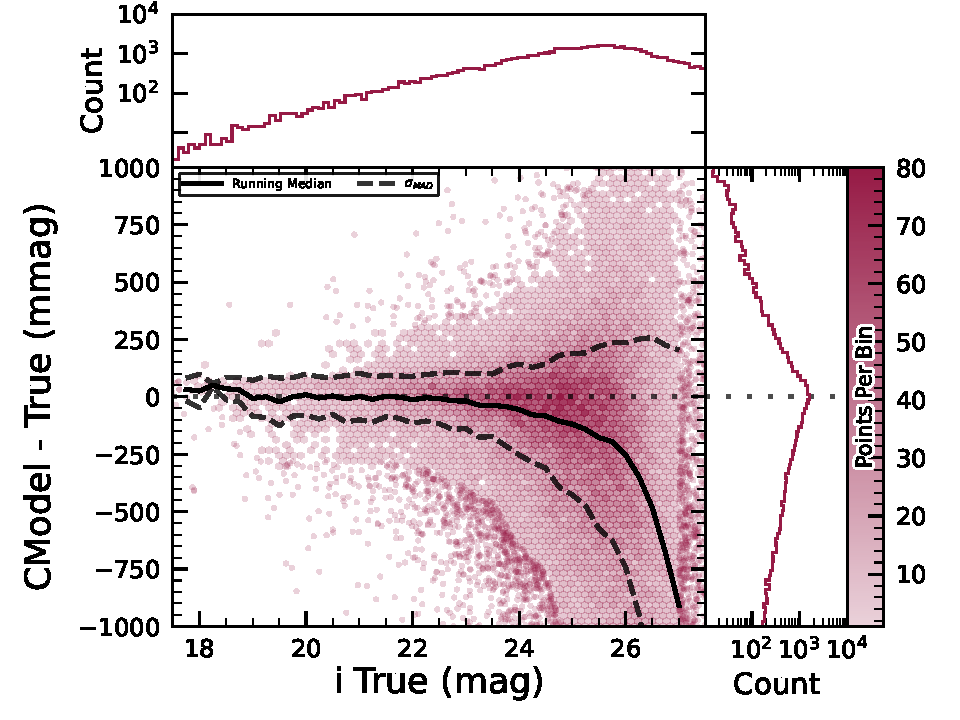
\includegraphics[width=\linewidth]{injected_lsst_cells_v1_5063_i_mag_cmodel}
  \caption{$i$-band magnitude residuals for CModel measurements of injected galaxies.}
  \end{subfigure}\hfill
  \begin{subfigure}[t]{0.45\textwidth}
  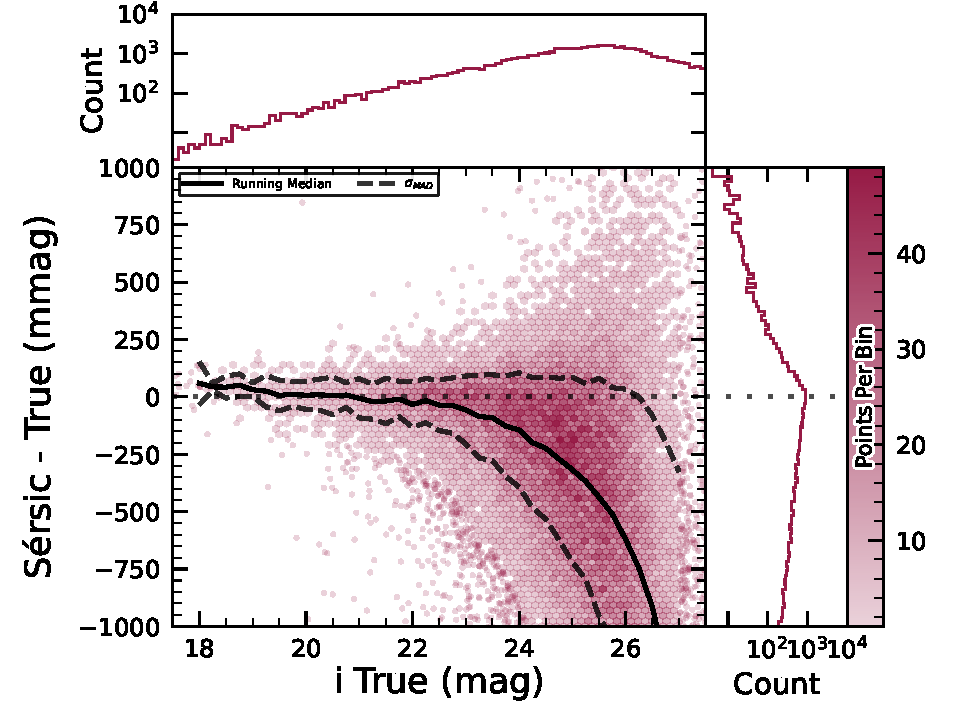
\includegraphics[width=\linewidth]{injected_lsst_cells_v1_5063_i_mag_sersic}
  \caption{$i$-band magnitude residuals for S\'ersic model measurements of injected galaxies.}
  \end{subfigure}\hfill
\caption{$i$-band magnitude residuals for matched injected DC2 galaxies with the CModel and S\'ersic algorithms in a portion of the \gls{ECDFS} region, including the median and scatter thereof.
The black line is the median.}
\label{fig:injected_lsst_cells_v1_5063_i_mag}
\end{figure*}
\figref{fig:injected_lsst_cells_v1_5063_r_color_g_minus_i} shows $g-i$ color residuals versus $r$-band magnitude for the same sample of galaxies as \figref{fig:injected_lsst_cells_v1_5063_i_mag}.
For this and most other colors, \gls{GAaP} (with a $1''$ aperture) and S\'ersic colors both yield lower scatter; however, the CModel colors have the smallest bias.
Curiously, the \gls{GAaP} bias appears to be magnitude-dependent, whereas the S\'ersic bias remains stable from $19<r<26$.
Any of these color measurements are suitable for use for deriving quantities like photometric redshifts, stellar population parameters, etc.

\begin{figure*}[hbt!]
  \centering
  \begin{subfigure}[t]{0.31\textwidth}
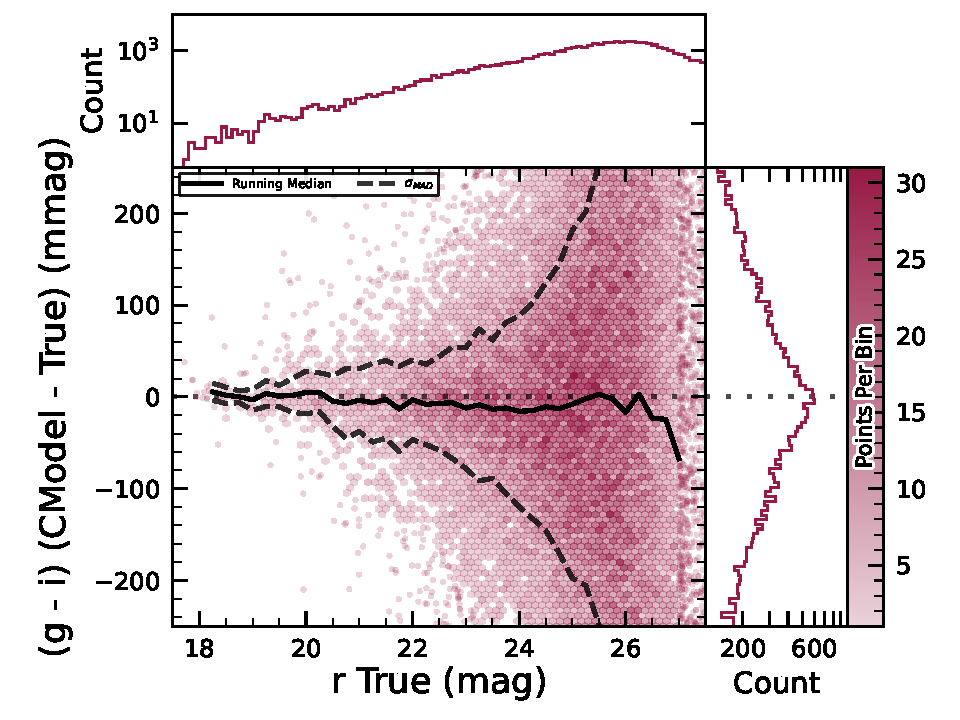
\includegraphics[width=\linewidth]{injected_lsst_cells_v1_5063_r_color_cmodel_g_minus_i}
  \caption{$g-i$ color residuals for CModel measurements of injected galaxies.}
  \end{subfigure}\hfill
  \begin{subfigure}[t]{0.31\textwidth}
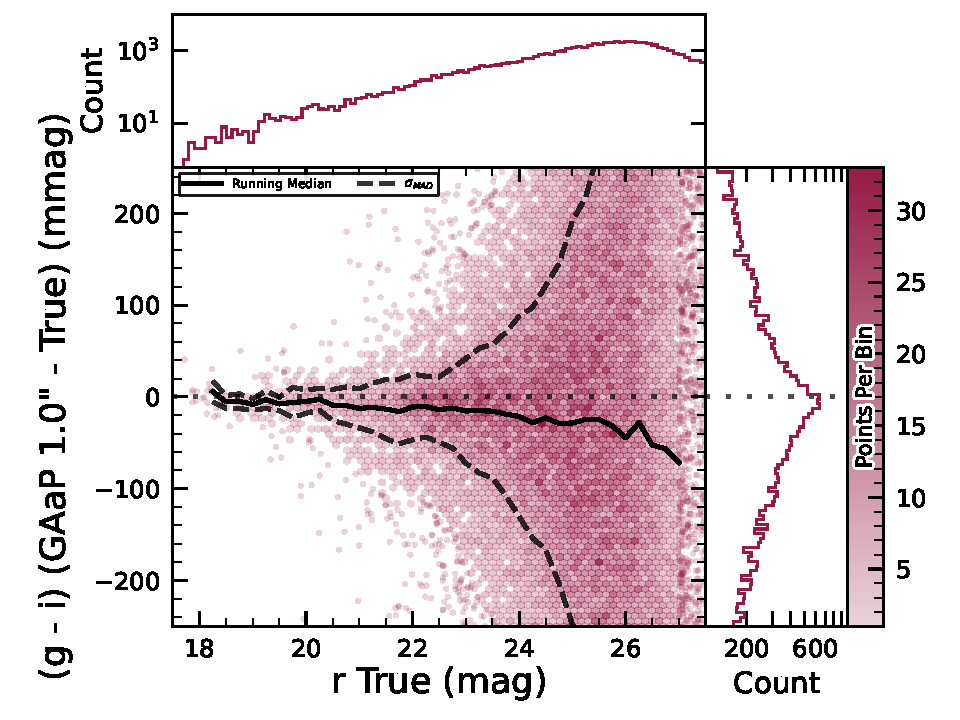
\includegraphics[width=\linewidth]{injected_lsst_cells_v1_5063_r_color_gaap_g_minus_i}
  \caption{$g-i$ color residuals for \gls{GAaP} measurements of injected galaxies.}
  \end{subfigure}\hfill
    \begin{subfigure}[t]{0.31\textwidth}
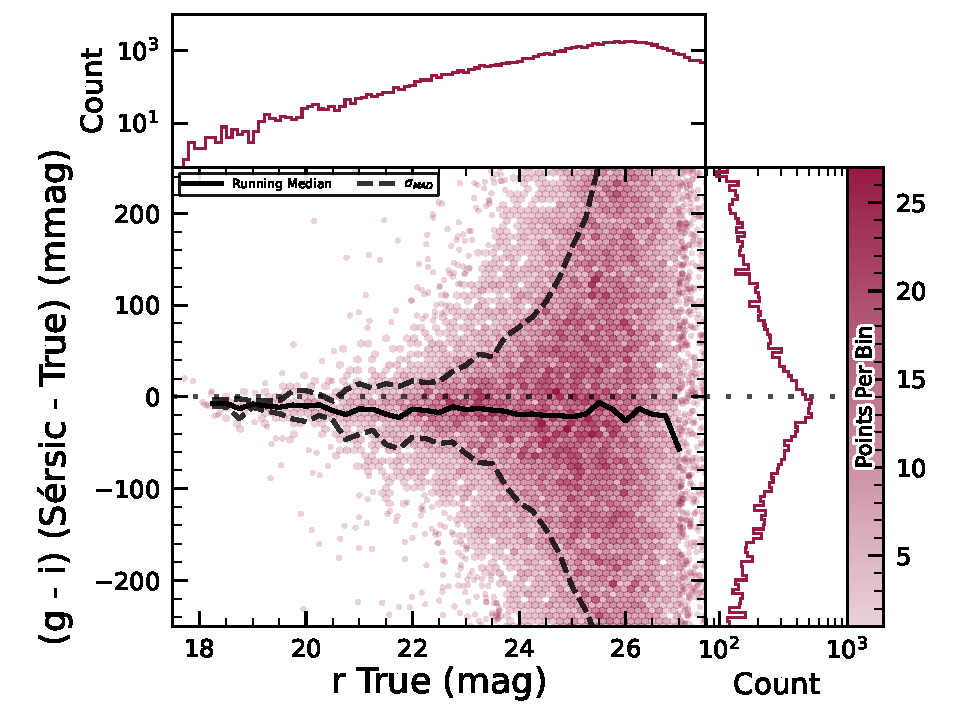
\includegraphics[width=\linewidth]{injected_lsst_cells_v1_5063_r_color_sersic_g_minus_i}
  \caption{$g-i$ color residuals for S\'ersic model measurements of injected galaxies.}
  \end{subfigure}\hfill
\caption{$g-i$ color residuals versus true $r$-band magnitude for matched injected DC2 galaxies with the CModel, \gls{GAaP} and S\'ersic algorithms in a portion of the \gls{ECDFS} region.}
\label{fig:injected_lsst_cells_v1_5063_r_color_g_minus_i}
\end{figure*}
In addition to photometry, some algorithms include measurements of structural parameters like size, ellipticity, and S\'ersic index.
One particular known issue is that many (truly) faint objects have significantly overestimated sizes and fluxes.
This was also seen in the Dark Energy Survey \citep{2025arXiv250105739B}, who dubbed such objects ``super-spreaders''.
These super-spreaders contribute significantly to overestimated fluxes at the faint end (see e.g. \figref{fig:injected_lsst_cells_v1_5063_i_mag}), and are particularly problematic for the Kron algorithm \citep{1980ApJS...43..305K}, which should only be used with caution.

As mentioned in \secref{ssec:coadd_processing}, the S\'ersic fits include a free centroid, which is initialized from the fiducial centroid of the object.
Preliminary analyses of matched injected objects suggest that the S\'ersic model galaxy \gls{astrometry} residuals are somewhat smaller than for the standard centroids used in other measurements, and so users of the S\'ersic photometry should also use these centroid values.
One caveat is that for faint objects and/or in crowded regions with unreliable deblending, free centroids can drift significantly and potentially towards other objects, so objects with large differences between the fiducial and S\'ersic \gls{astrometry} should be discarded or used with caution.

S\'ersic model parameter uncertainties are estimated by computing and inverting the Hessian matrix with the best-fit parameter values, after replacing the pixel data (but not uncertainties) by the best-fit model values.
Currently, only the on-diagonal dispersion term (square root of the variance) is provided as an error estimate for each parameter.
Future releases may provide more off-diagonal terms of the covariance matrix - particularly for the structural parameters, which are known to be correlated.

A major outstanding issue is that many parameter uncertainties - including but not limited to those for fluxes - are underestimated.
This is at least partly (but not wholly) due to the fact that coaddition introduces covariance between pixels, which is not captured in per-pixel variances.

\begin{figure*}[hbt!]
  \centering
  \begin{subfigure}[t]{0.45\textwidth}
  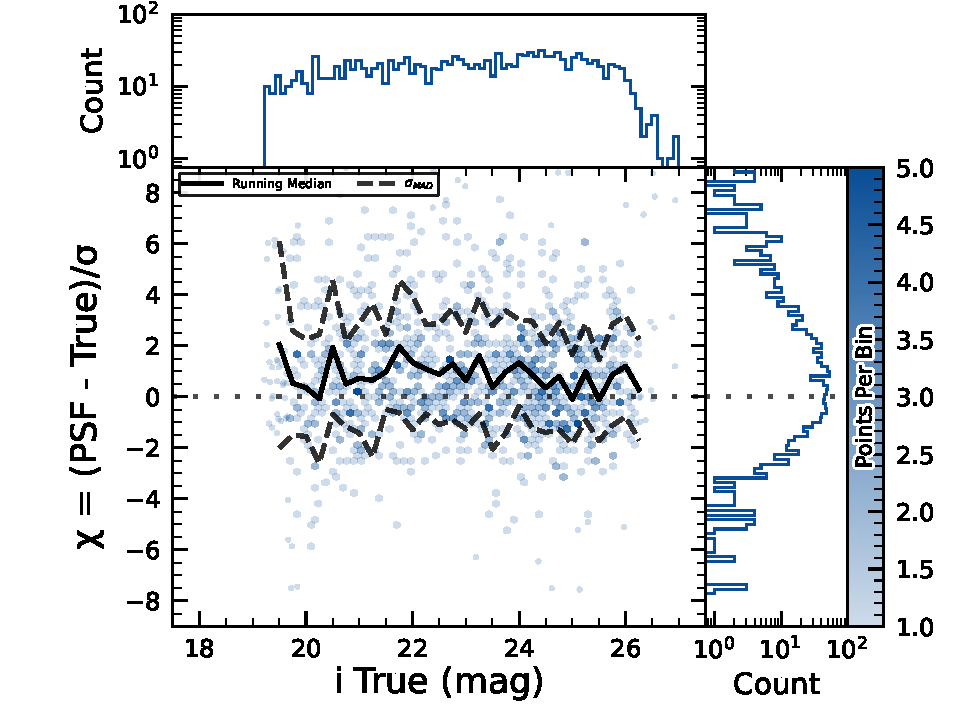
\includegraphics[width=\linewidth]{injected_lsst_cells_v1_5063_i_mag_chi_psf}
  \caption{$i$-band flux uncertainty-scaled residuals for PSF model measurements of injected stars.}
  \end{subfigure}\hfill
  \begin{subfigure}[t]{0.45\textwidth}
  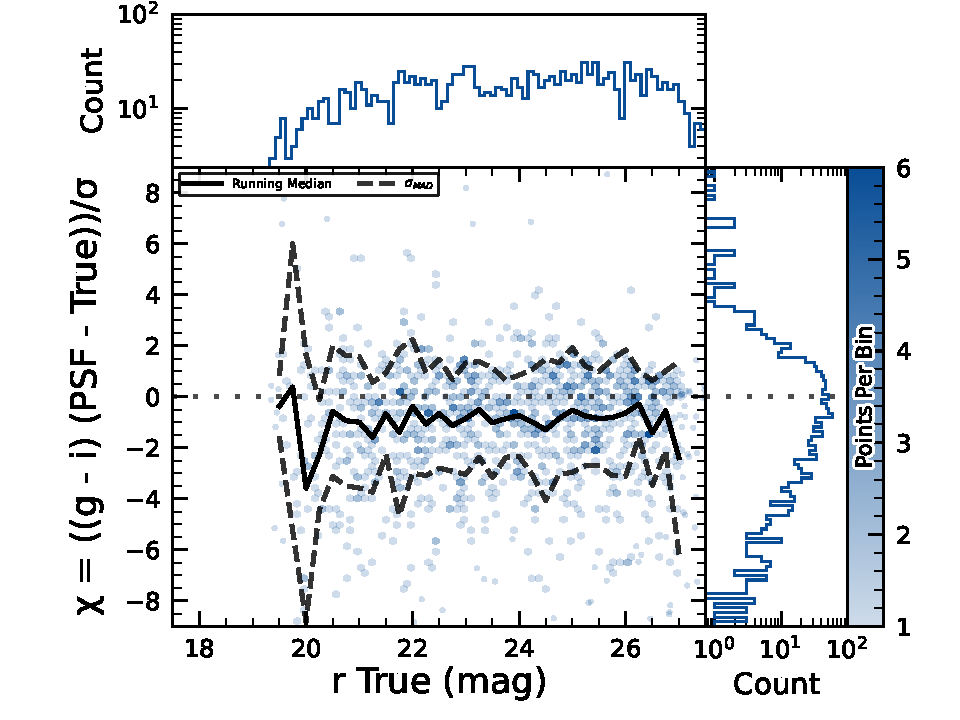
\includegraphics[width=\linewidth]{injected_lsst_cells_v1_5063_r_color_chi_psf_g_minus_i}
  \caption{$g-i$ color uncertainty-scaled residuals for PSF model measurements of injected stars.}
  \end{subfigure}\hfill
\caption{Color and flux uncertainty-scaled residuals for matched injected DC2 stars' PSF model measurements in a portion of the \gls{ECDFS} region.}
\label{fig:injected_lsst_cells_v1_5063_star_psf_chi}
\end{figure*}

The degree to which uncertainties are underestimated can depend on the parameter in question and on the brightness of the object.
In plots of uncertainty-scaled residuals, the ideal behavior is for the median (i.e. the bias) to lie close to zero, and for the $\pm1\sigma$ lines to lie at $\pm1$, without any dependence on magnitude.
\figref{fig:injected_lsst_cells_v1_5063_star_psf_chi} shows that flux and color uncertainties for PSF model magnitudes of injected stars are both underestimated, but by a factor of approximately $1.7-2$ that is not very sensitive to \gls{SNR}.
This holds for astrometric/centroid parameters as well.

\begin{figure*}[hbt!]
  \centering
  \begin{subfigure}[t]{0.45\textwidth}
  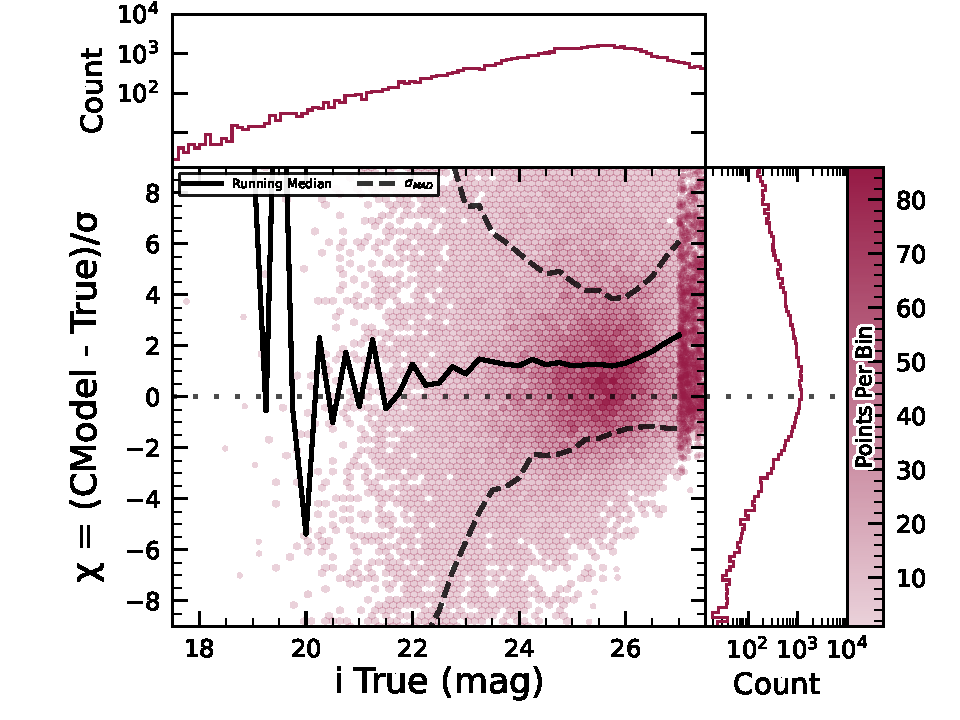
\includegraphics[width=\linewidth]{injected_lsst_cells_v1_5063_i_mag_chi_cmodel}
  \caption{$i$-band flux uncertainty-scaled residuals for CModel measurements of injected galaxies.}
  \end{subfigure}\hfill
  \begin{subfigure}[t]{0.45\textwidth}
  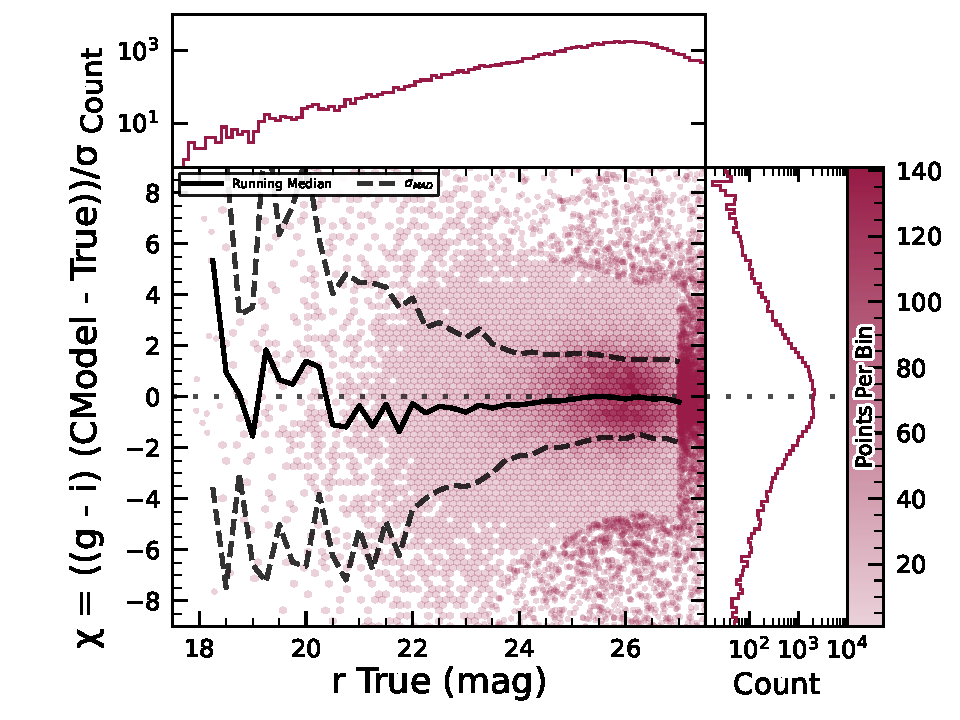
\includegraphics[width=\linewidth]{injected_lsst_cells_v1_5063_r_color_chi_cmodel_g_minus_i}
  \caption{$g-i$ color uncertainty-scaled residuals for CModel measurements of injected galaxies.}
  \end{subfigure}\hfill
\caption{Color and flux uncertainty-scaled residuals for matched injected DC2 galaxies' CModel measurements in a portion of the \gls{ECDFS} region.}
\label{fig:injected_lsst_cells_v1_5063_galaxy_cmodel_chi}
\end{figure*}

\begin{figure*}[hbt!]
  \centering
  \begin{subfigure}[t]{0.45\textwidth}
  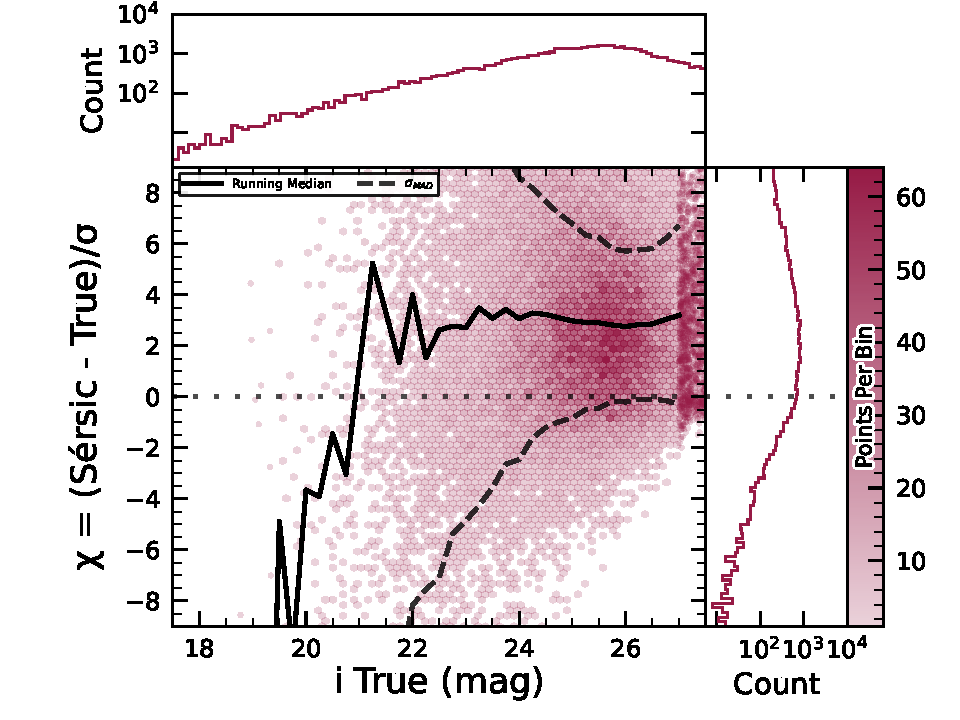
\includegraphics[width=\linewidth]{injected_lsst_cells_v1_5063_i_mag_chi_sersic}
  \caption{$i$-band flux uncertainty-scaled residuals for S\'ersic model measurements of injected galaxies.}
  \end{subfigure}\hfill
  \begin{subfigure}[t]{0.45\textwidth}
  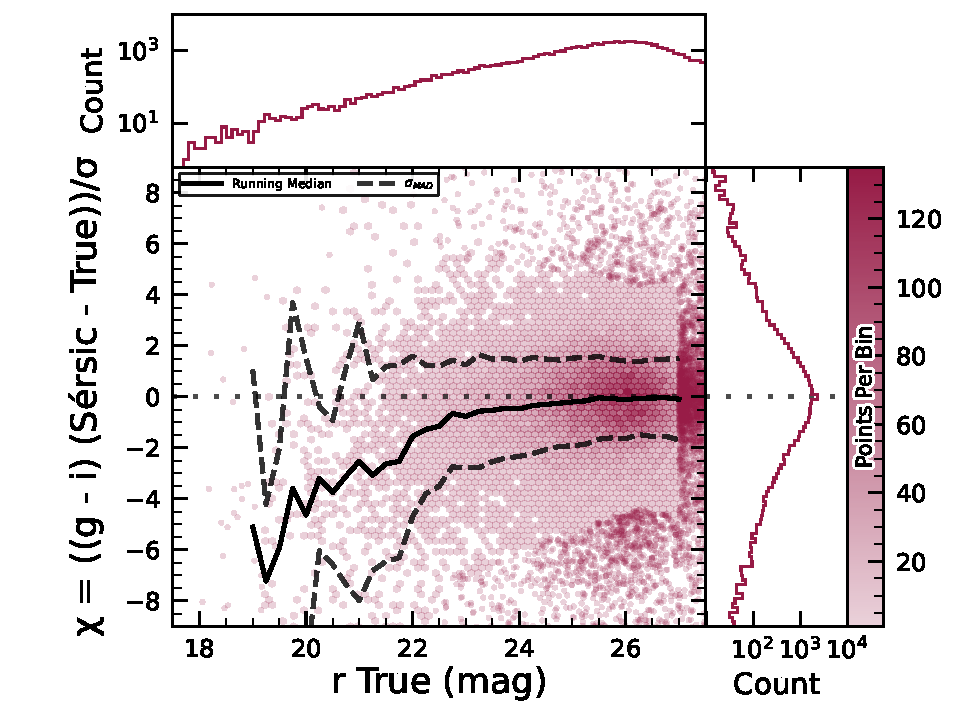
\includegraphics[width=\linewidth]{injected_lsst_cells_v1_5063_r_color_chi_sersic_g_minus_i}
  \caption{$g-i$ color uncertainty-scaled residuals for S\'ersic model measurements of injected galaxies.}
  \end{subfigure}\hfill
\caption{Color and flux uncertainty-scaled residuals for matched injected DC2 galaxies' S\'ersic measurements in a portion of the \gls{ECDFS} region.}
\label{fig:injected_lsst_cells_v1_5063_galaxy_sersic_chi}
\end{figure*}

In turn, \figref{fig:injected_lsst_cells_v1_5063_galaxy_cmodel_chi} shows that CModel color uncertainties of galaxies are underestimated by a similar factor at the faint end, but with appreciable scaling with magnitude (and thereby \gls{SNR}).
Flux error underestimation is both larger than for colors and scales more strongly with \gls{SNR}.
This indicates that systematic effects dominate the errors in fluxes, particularly for bright galaxies.
This is also at least partly but not wholly due to so-called model inadequacy - that is, the fact that galaxy models, parameteric or otherwise, are insufficiently complex to capture the structure of real galaxies.

\figref{fig:injected_lsst_cells_v1_5063_galaxy_sersic_chi} shows that S\'ersic model fluxes and colors have similar behavior as CModel, but with a greater degree of overestimation.
This may be partly due to the fact that S\'ersic parameter uncertainties are estimated along with the free centroid and structural (shape and S\'ersic index) parameters, whereas the forced CModel fluxes and errors are derived from linear flux fits with a fixed shape and centroid.

Efforts are underway to investigate and quantify the origin of uncertainty underestimates and future releases will, at the least, provide recommendations for mitigations.

\subsection{Difference Imaging Purity} 
\label{sec:performance:dia}

We assessed the performance of image differencing using human vetting and source injection (\S \ref{sec:perf:dia_completeness}).
Members of the \gls{DP1} team labeled more than 9500 DIASource image triplets consisting of cutouts from the science, template, and difference images.
We classified these into various real and artifact categories.
The raw artifact to real ratio without filtering was roughly 9:1.
Bright stars are the main source of artifacts.
Correlated noise, primarily in $u$ and $g$ bands, also leads to spurious detections near the flux threshold.
We expect to be able to mitigate these effects for \gls{LSSTCam}.

Applying a reliability threshold improves the purity of transients but not variable stars; technical limitations at the time of model training prevented injection of variable stars into the synthetic training set.
Reliability models, described in \secref{ssec:diffim_analysis},  for \gls{LSSTCam} data will be trained on a wider range of input data.

\subsection{Difference Imaging Detection Completeness} \label{sec:perf:dia_completeness}

We assess the performance of our difference imaging \gls{pipeline} using synthetic source injection on the science images prior to differencing.
We construct a catalog of injected sources by joining two different samples of point sources, a set of hosted sources to emulate transients in galaxies and second set of hostless sources.
The hosts are selected from the pipeline source catalog that is produced upstream by imposing a cut on their extendedness measurement and selecting $N_{\rm src}={\rm min}(100, N\times0.05)$ of the $N$ available sources per detector.
For each host we pick a random position angle and radius using its light profile shape to decide where to place the source, and also a random value of brightness for the injected source, with magnitudes higher than the host source.

The hostless sources instead have random positions in the \gls{CCD} focal plane, and magnitudes chosen 
from a random uniform distribution with $20 \geq m \geq m_{lim} + 1$,  where $m_{lim}$ is the limiting magnitude of the image.
We used the \gls{LSST}  \texttt{source\_injection} package\footnote{\url{https://pipelines.lsst.io/modules/lsst.source.injection/index.html}} to include these sources in our test images.
We performed a coordinate cross-match task, with a threshold of $0\farcs5$ to find which of these sources were detected and which were lost, enabling the calculation of a set of performance metrics.

In \figref{fig:eff_snr_griz} we show the detection completeness as a function of the \gls{SNR}, for sources in the \gls{ECDFS} field, for filters $griz$. 
We observe a completeness $>95\%$ for sources with \gls{SNR}$> 6$, with mean completeness $\simeq 99\%$ and standard deviation of $\simeq 0.7\%$.
%
\begin{figure}[htb!]
\plotone{efficiency_snr_griz}
\caption{The difference image detection completeness for injected sources in the \gls{ECDFS} field, for filters \textit{griz}, as a function of the estimated signal to noise ratio SNR. 
This completeness is the ratio between the found fake sources (shaded histogram) and all the sources (solid line). 
The horizontal dashed line represents where the $50\%$ completeness level is reached, at approximately SNR $\simeq 5.07$.}
\label{fig:eff_snr_griz}
\end{figure}
%
In \figref{fig:coordinate_offset_diffim_fakes} we show the distribution of the residuals of the recovered sky coordinates for the detected synthetic sources. The marginal distributions are both centered at zero, and for sources of SNR $>20$ the residuals are compatible with normal distributions $\mathcal{N}(\mu=0, \sigma^2=(0''.02)^2)$.
%
\begin{figure}[htb!]
\plotone{coordinate_offsets_hexbin}
\caption{Coordinate residuals for detected synthetic sources in difference images, between recovered and true position of the sources in the \gls{ECDFS} field. 
In the top and right panels we include the distribution of these offsets, for all sources as well as for sources with SNR$>20$. 
These high SNR sources show gaussian coordinate residual distributions with $\sigma=0\farcs02$ (black solid lines). 
The circle reflects the matching radius of $0\farcs5$.}
\label{fig:coordinate_offset_diffim_fakes}
\end{figure}
%
In \figref{fig:phot_residual_diffim_fakes} we show photometry results for our detected synthetic sources in the \textit{i} filter, using \gls{PSF} photometry on the difference images. 
We include both the magnitude residuals as well as the flux pulls, defined as $f_{PSF}-f_{\rm{True}})/\sigma_{f_{PSF}}$ for PSF \gls{flux} $f_{PSF}$ and error $\sigma_{f_{PSF}}$,  
as a function of the true magnitude of the synthetic sources, including the running median and median absolute deviation (MAD) for the whole brightness range. 
We also include the true magnitude distribution as well as the detection completeness on the top panel, and for reference the $90\%$ and $50\%$ completeness magnitude values in vertical lines. 
On the right panels we include the marginal distribution for sources brighter than $mag < 22.5$, splitting the data into hosted and hostless, as well as the robust mean and standard deviation.
%
From this figure we can see that our \gls{flux} measurements are accurate within a wide range of magnitudes, for both hosted and hostless synthetic sources. 
We find that the median offset is below $0.002$ mag for true magnitudes below $21$, and with a maximum $\sigma_{MAD}$ scatter of about $0.02$ mag in this range.
For true $m_i < 22.5$, the robust running median PSF magnitudes residuals are $<0.02$ mag, and when splitting into hosted and hostless both robust median
are well below $0.01$, and robust $\sigma$, i.e. $\sigma_{MAD}$ are also well below $0.05$.
%
For all sources with $m_i<21.5$ the running median is always $|\left<\delta\right>| <0.1$, and MAD $\sigma_\delta < 1$. 
Extending to sources with $m_i<22.5$ then  hostless sources have  a robust mean pull below $0.02$, with a robust standard deviation $<1.15$, while these parameters increase to $0.2$ and $1.2$ for hosted sources, suggesting that we might have contamination from host background sources potentially biasing our fluxes.
%
\begin{figure}
\plotone{hexbin_psf_magpull}
\caption{Magnitude residuals and flux pulls for $i$-band \gls{PSF} photometry on difference images for ECDFS field in $i$ for detected injected sources.
Top panel: Distribution of true magnitudes for injected sources (blue), and split  into hostless (black dash) and hosted (orange) sources, with detection completeness as a function of true magnitude (gray line). 
Vertical dashed lines indicate the 90\% and 50\% completeness magnitude limits.
Center left panel: 2D hexbin plot of PSF magnitude residuals (measured minus true) versus true magnitude for detected sources, with running median (solid black) and $\sigma_{MAD}$ (dashed black) overlaid.
Center right panel: Marginalized distributions of PSF magnitude residuals for hostless (blue) and hosted (orange) sources with true magnitude $m_i < 22.5$, annotated with robust mean and standard deviation. 
Bottom left panel: 2D hexbin plot of PSF flux pulls versus true magnitude for detected sources, with running median (solid black) and $\sigma_{MAD}$ (dashed black) overlaid.
Bottom right panel: Marginalized distributions of PSF flux pulls for hostless (blue) and hosted (orange) sources with true magnitude $m_i < 22.5$, annotated with robust mean and standard deviation.}
\label{fig:phot_residual_diffim_fakes}
\end{figure}
%
\subsection{Solar System}
\label{sec:performance:solsys}

\subsubsection{Asteroid Linking Performance}

The evaluation of asteroid linking performance in DP1 focused on demonstrating discovery capability.
The solar system discovery pipeline produced 269,581 tracklets, 5,691 linkages, and 281 post-processed candidates.

As described in \secref{sec:drp:solsys}, post-processing of the \texttt{heliolinc} output with \texttt{link\_purify} produced a final set of 281 candidate linkages, ranked with the most promising first. 
We then used \texttt{find\_orb} \citep{findorb} to derive orbit fits for each candidate, sorting the resulting list by $\chi\_{\rm dof}^2$, a measure of fit quality. 
A conservative manual investigation of these candidates yielded a curated list of \nnewasteroiddiscoveries probable new asteroid discoveries.
Manual inspection of the linkages indicated that those ranked 0--137 corresponded to unique real asteroids; ranks 138--200 contained additional real objects intermixed with some spurious linkages; and ranks higher than 200 were essentially all spurious.
This analysis indicates that it will be possible to identify cuts on quality metrics such as $\chi^2$ to define discovery candidate samples with high purity; determining the exact quantitative cut values requires more data with \gls{LSSTCam}.
We next removed all observations matched to known asteroids (using \gls{MPC}'s MPChecker service), reducing the number of candidates to 97.
Of these, four had strong astrometric and/or photometric outliers, likely due to self-subtraction in difference images due to the unavoidable limitations of template generation from the limited quantity of data available from  \gls{LSSTComCam}.
We suspect these four linkages do correspond to real objects, but have chosen to discard them out of an abundance of caution.
The remaining \nnewasteroiddiscoveries were submitted to the Minor Planet Center and accepted as  discoveries, demonstrating the \gls{LSST} pipelines are able to successfully discover new solar system objects.

\subsubsection{Asteroid Association Performance}
\label{ssec:asteroid_association}

During the Solar System association step,  \nsolarsystemsources \textit{DiaSources} were linked to \nsolarsystemobjects  unique Solar System objects, 
These include 3,934 \textit{DiaSources} with 338 previously known objects cataloged by the \gls{MPC}, and 2,054 \textit{DiaSources} with the \nnewasteroiddiscoveries  newly-discovered objects. 
An additional 143 detections of these newly discovered objects were also recovered. 
These detections were not initially identified by the discovery pipelines, as they did not meet the required criteria for tracklet formation, specifically the minimum number of detections and/or the maximum allowed time span between observations.

\begin{figure}[htb!]
\plotone{sso_residuals}
\caption{Astrometric residuals between expected and observed positions of Solar System Objects in \gls{DP1}. 
The median residuals are $0\farcs001$ and $-0\farcs016$ in R.A./Dec direction, with  standard deviations of $0.''19$ and $0.''10$, respectively. 
No detectable systematic offset from zero indicates there are no major errors in either timing or astrometry delivered by the Rubin system. 
The wider scatter in the RA direction is due to objects whose measured orbital elements are less well constrained, translating to larger along-track positional errors in the predicted positions.}
\label{fig:sso_residuals}
\end{figure}

The astrometric residuals of known asteroid associations are shown in \figref{fig:sso_residuals}.
The astrometric precision for solar system sources is excellent, with the majority of objects detected within $0\farcs1$ of their expected positions.
Taking the signed median residuals to search for biases, we find that previously-known objects have mean residuals of $0\farcs001$ and $-0\farcs016$ in the RA and Dec directions respectively, while newly-discovered objects have mean residuals of $-0\farcs035$ and $-0\farcs010$ in the RA and Dec directions, respectively.
These mean residuals are small enough to eliminate the possibility of a timing offset greater than the second-scale shutter motion, which is consistent with the timing studies presented in Section~\ref{ssec:comcam_timing}.

\subsection{Crowded Fields}
Among the seven Rubin DP1 target fields, two stand out for their severe stellar crowding: the globular cluster 47\,Tucanae (47\_Tuc) and the Fornax dwarf spheroidal galaxy (Fornax dSph).
These fields were selected in part to stress-test the LSST Science Pipelines under high-density conditions. 
While both exhibit high stellar densities, the nature and spatial extent of the crowding differ significantly.

47\,Tuc presents extreme crowding across much of the field, encompassing its dense core and the eastern regions influenced by the Small Magellanic Cloud (SMC). 
This pervasive crowding leads to persistent challenges for deblending and reliable source detection, exposing field-wide limitations in the current pipeline performance \citep{Choi2025}.
In contrast, Fornax\,dSph shows significant crowding only in its central region, with outer areas remaining well resolved and easier to process. 

In both 47\,Tuc and Fornax, extreme crowding led to the deblending step being skipped frequently when memory or runtime limits were exceeded, typically due to an excessive number of peaks, or large parent footprints.
However, the impact of these limitations differed: in 47\,Tuc, deblending was often skipped across the entire field, resulting in large gaps and substantially reduced completeness. 
In Fornax, these issues were largely confined to the central region, with much better recovery in the outskirts. 
This contrast highlights how the pipeline’s limitations depend on the spatial extent of high-density regions: 47\,Tuc exposed systematic, field-wide challenges, whereas Fornax revealed more localized, density-driven limits.

\citet{Wainer2025} explored the Rubin DP1 \texttt{DiaObject} catalog (\secref{ssec:catalogs}) in the 47\,Tuc field, which contains sources detected in difference images. 
Because forced photometry is performed at these positions across all single-epoch images, this dataset bypasses the coadd-based detection and deblending stages that often fail in crowded regions. 
By computing the median of the forced photometry for each  \texttt{DiaObject} across available visits, they recovered approximately three times more candidate cluster members than found in the standard \texttt{Object table} \citep{Choi2025}. 
This result underscores the value of difference-imaging–based catalogs for probing dense stellar regions inaccessible to standard coadd processing in DP1.

Although the DP1 pipeline was not optimized for crowded-field photometry, these early studies of 47\,Tuc and Fornax provide critical benchmarks. 
They highlight both the limitations and opportunities for science with Rubin data in crowded environments, and they inform future pipeline development aimed at robust source recovery in complex stellar fields.
